\section{Period at 50 THz}

\subsection*{Resources}
\begin{itemize}
    \item Book: 1.2 (\url{https://see.stanford.edu/materials/lsoftaee261/book-fall-07.pdf})
    \item Video: Lecture 2 (\url{https://www.youtube.com/watch?v=1rqJl7Rs6ps})
\end{itemize}

\subsection*{Challenge}
A signal is oscillating at a frequncy of 50 THz.  What is the period?

\subsection*{Solution}
\six{s}

\hash{q}{33efc2}




%%%%%%%%%%%%%%%%%%%%%%%%%%%%%%%%%
\newpage
%%%%%%%%%%%%%%%%%%%%%%%%%%%%%%%%%

\section {Fundamental period with k=1}

\subsection*{Resources}
\begin{itemize}
    \item Book: 1.3 (\url{https://see.stanford.edu/materials/lsoftaee261/book-fall-07.pdf})
    \item Video: Lecture 2 (\url{https://www.youtube.com/watch?v=1rqJl7Rs6ps})
\end{itemize}

\subsection*{Challenge}
What is the fundamential period of $sin(2 \pi k t)$, where $t$ is time in seconds and $k=1$?

\subsection*{Solution}
\six{s}

\hash{w}{9ae2db}




%%%%%%%%%%%%%%%%%%%%%%%%%%%%%%%%%
\newpage
%%%%%%%%%%%%%%%%%%%%%%%%%%%%%%%%%

\section{Frequency with k=1}

\subsection*{Resources}
\begin{itemize}
    \item Book: 1.3 (\url{https://see.stanford.edu/materials/lsoftaee261/book-fall-07.pdf})
    \item Video: Lecture 2 (\url{https://www.youtube.com/watch?v=1rqJl7Rs6ps})
\end{itemize}

\subsection*{Challenge}
What is the frequency of $sin(2 \pi k t)$, where $t$ is time in seconds and $k=1$?

\subsection*{Solution}
\six{Hz}

\hash{e}{453c99}




%%%%%%%%%%%%%%%%%%%%%%%%%%%%%%%%%
\newpage
%%%%%%%%%%%%%%%%%%%%%%%%%%%%%%%%%

\section{Frequency with k=2}

\subsection*{Resources}
\begin{itemize}
    \item Book: 1.3 (\url{https://see.stanford.edu/materials/lsoftaee261/book-fall-07.pdf})
    \item Video: Lecture 2 (\url{https://www.youtube.com/watch?v=1rqJl7Rs6ps})
\end{itemize}

\subsection*{Challenge}
What is the frequency of $sin(2 \pi k t)$, where $t$ is time in seconds and $k=2$?

\subsection*{Solution}
\six{Hz}

\hash{r}{111802}




%%%%%%%%%%%%%%%%%%%%%%%%%%%%%%%%%
\newpage
%%%%%%%%%%%%%%%%%%%%%%%%%%%%%%%%%

\section{Fundamental period with k=2}

\subsection*{Resources}
\begin{itemize}
    \item Book: 1.3 (\url{https://see.stanford.edu/materials/lsoftaee261/book-fall-07.pdf})
    \item Video: Lecture 2 (\url{https://www.youtube.com/watch?v=1rqJl7Rs6ps})
\end{itemize}

\subsection*{Challenge}
What is the fundamental period of $sin(2 \pi k t)$, where $t$ is time in seconds and $k=2$?

\subsection*{Solution}
\six{s}

\hash{t}{c4c8be}




%%%%%%%%%%%%%%%%%%%%%%%%%%%%%%%%%
\newpage
%%%%%%%%%%%%%%%%%%%%%%%%%%%%%%%%%

\section{Fundamental period with multiple terms}

\subsection*{Resources}
\begin{itemize}
    \item Book: 1.3-1.4 (\url{https://see.stanford.edu/materials/lsoftaee261/book-fall-07.pdf})
    \item Video: Lecture 2 (\url{https://www.youtube.com/watch?v=1rqJl7Rs6ps})
\end{itemize}

\subsection*{Comments}
So $k$ here is proportional to the frequency. Double $k$ and the frequency doubles. Every ``step'' around the circle drawn by the sine curve becomes 2 steps when $k=2$, so within half the time you are already one time around the circle for $k=2$, and thus the number of times you go around the circle during one second (measured with $t$) is twice rather than once. $k$ is also inversely proportional to the period. Since with $k=2$ every ``step'' is now twice as large, so one completes the circle in half the time.

Even with multiple terms (frequencies), the period of the composite signal is always that of the highest (longest) period (lowest frequency), even if it is composed of multiple frequencies. You have to wait for every part of the signal to complete before a single period is complete. Ie, it is possible to add new frequencies to a signal without the period changing.

\subsection*{Challenge}
What is the fundamental period of $sin(2 \pi t) + sin(4 \pi t)$, where $t$ is time in seconds?

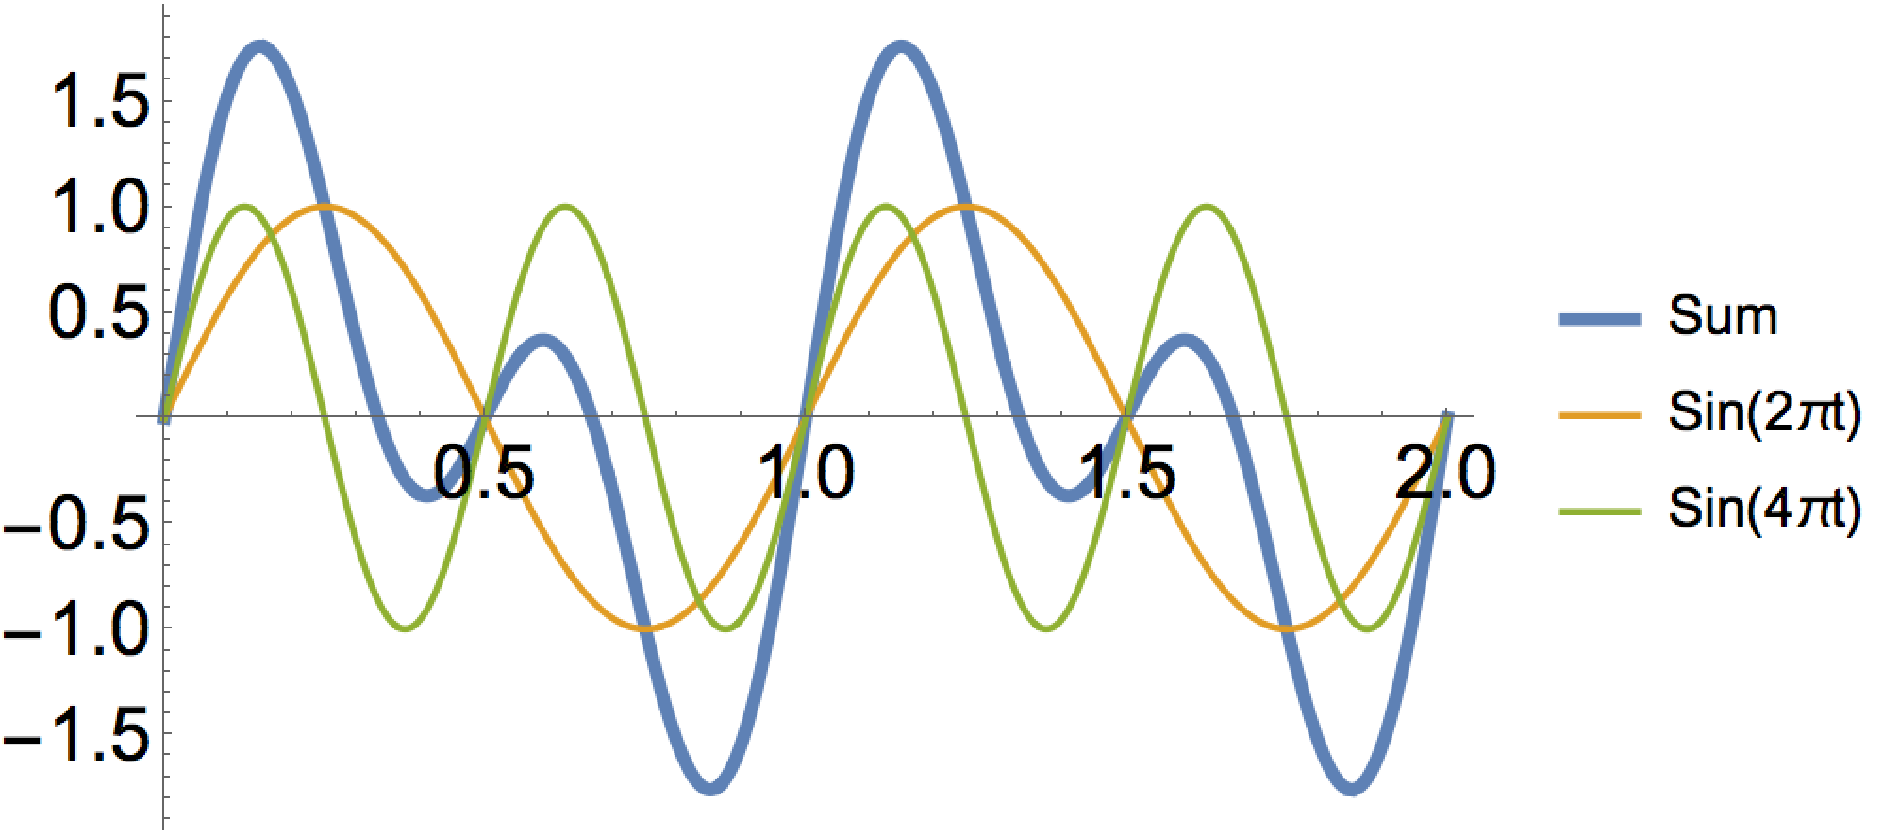
\includegraphics{period_with_multiple_terms.png}

\subsection*{Solution}
\six{s}

\hash{y}{80681b}




%%%%%%%%%%%%%%%%%%%%%%%%%%%%%%%%%
\newpage
%%%%%%%%%%%%%%%%%%%%%%%%%%%%%%%%%
\section{Amplitude}

\subsection*{Resources}
\begin{itemize}
    \item Book: 1.3 (\url{https://see.stanford.edu/materials/lsoftaee261/book-fall-07.pdf})
    \item Video: Lecture 2 (\url{https://www.youtube.com/watch?v=1rqJl7Rs6ps})
\end{itemize}

\subsection*{Comments}
Another important concept is amplitude. $Sin(2 \pi t)$ has an amplitude of 1, but this can be easily modified to go between $\pm A$ by multiplication with $A$.

\subsection*{Challenge}

The following 4 graphs are of the form $A Sin(2 \pi k t)$ with variation in the values of $A$ and $k$ \emph{only}. What is the sum of the values of $A$ for the following graphs? 

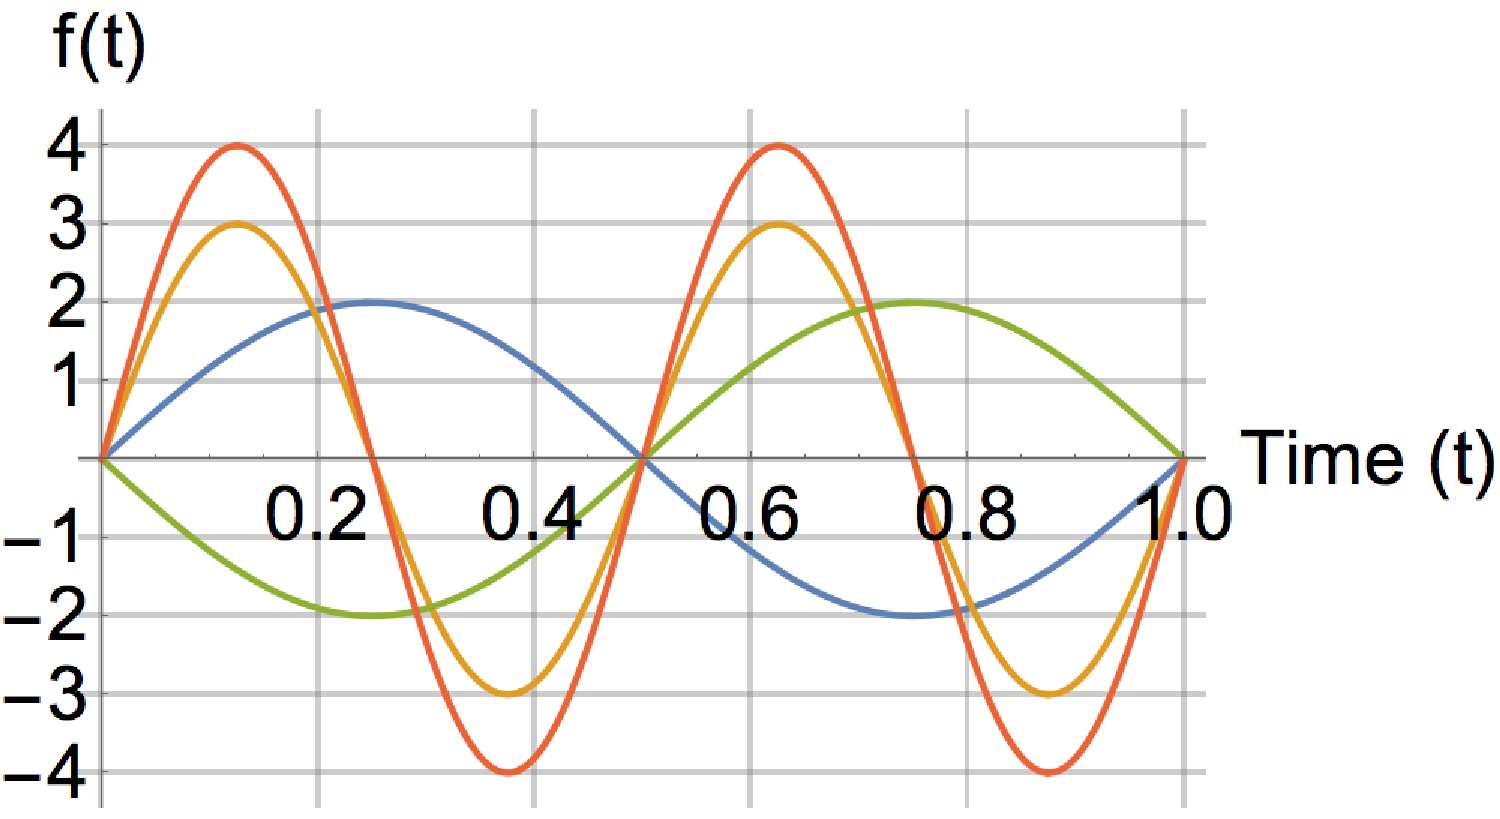
\includegraphics{amplitude.png}

\subsection*{Solution}
X

\hash{u}{7bcfe4}




%%%%%%%%%%%%%%%%%%%%%%%%%%%%%%%%%
\newpage
%%%%%%%%%%%%%%%%%%%%%%%%%%%%%%%%%

\section{Phase}

\subsection*{Resources}
\begin{itemize}
    \item Book: 1.3 (\url{https://see.stanford.edu/materials/lsoftaee261/book-fall-07.pdf})
    \item Video: Lecture 2 (\url{https://www.youtube.com/watch?v=1rqJl7Rs6ps})
\end{itemize}

\subsection*{Comments}
Another important concept is phase. For a simple Sine signal $\theta(t) = sin(2 \pi t)$, at $t=0$ the angle $\theta$ is zero, but one can shift the phase (starting point) of the signal by effectively making the sine-curve non-zero at $t=0$. Another way to think about it is to say the sine curve doesn't reach zero until a time $t-\phi$ where $\phi$ is the phase-shift added.

\subsection*{Challenge}

The following 4 graphs are of the form $Sin(2 \pi t + \phi)$ where $\phi$ is the phase-shift. Put the graphs in order corresponding to the following order of phase-shifts: $\pi/2$, $-\pi/2$, $\pi/4$, $2 \pi$.

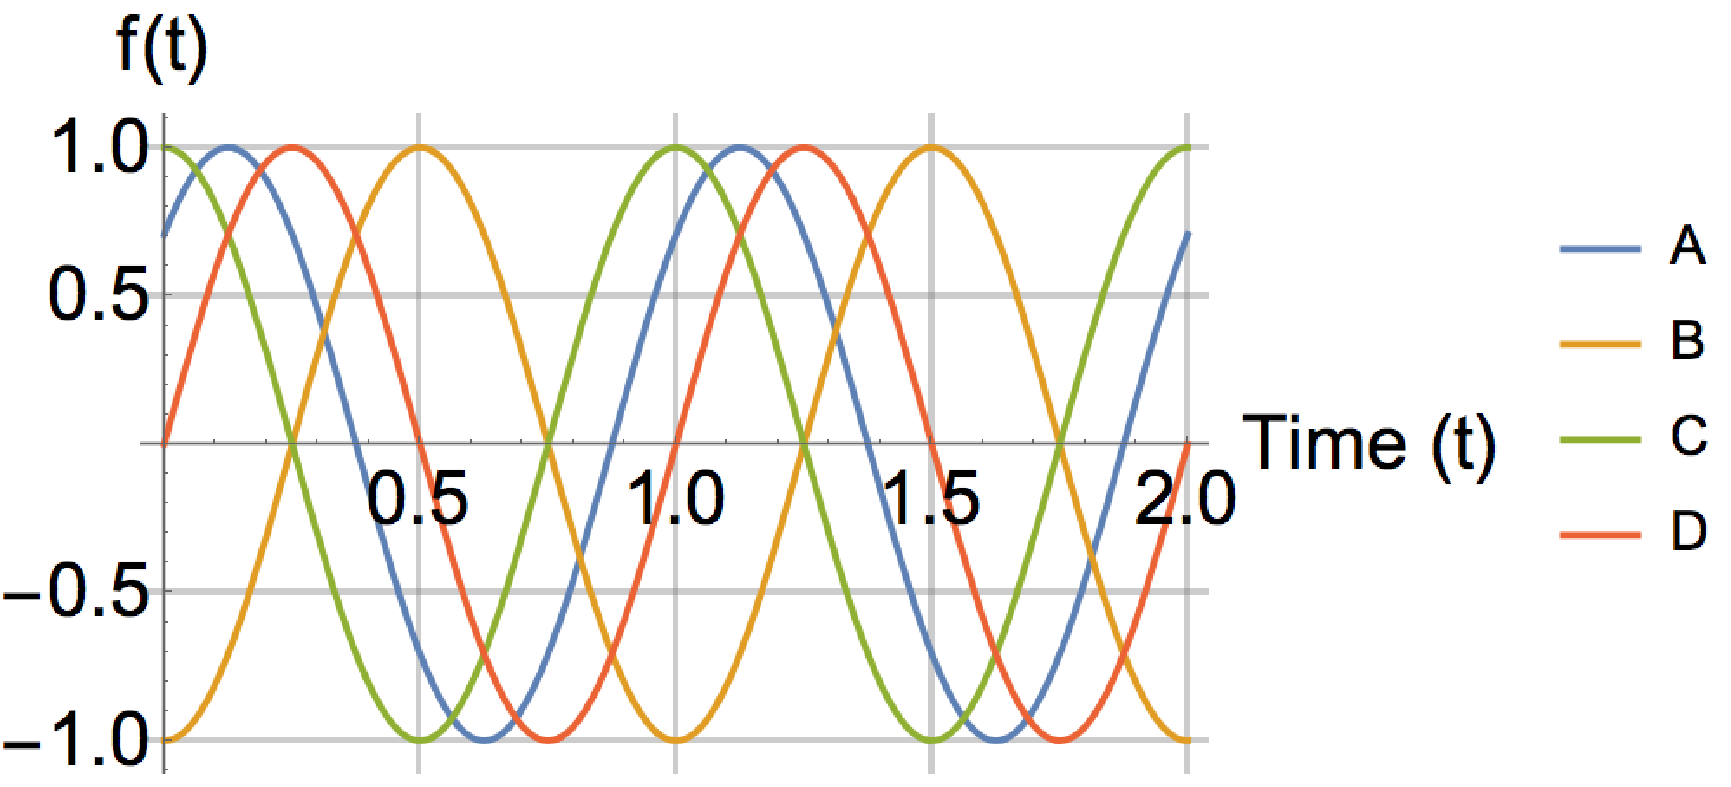
\includegraphics{phase_shift.png}

\subsection*{Solution}
X

\hash{i}{0efd66}
